%
% Chessboard calibration pattern generator
% Board size, colors and auxilary printing is configurable from within the script.
%
% 2020, christoph.heindl@gmail.com, https://github.com/cheind/

\documentclass[tikz]{standalone}
\usepackage{pst-calculate}
\newif\ifprintdims
\newif\ifprintcontrols

% Parameters
\def\N{8}                                   % number of inner corners in X-dir
\def\M{5}                                   % number of inner corners in Y-dir
\def\S{6.8}                                 % unit-less length of square
\def\U{cm}                                  % units
\definecolor{fgcolor}{cmyk}{60,40,40,100}   % rich black as foreground color
\definecolor{bgcolor}{cmyk}{0,0,0,0}        % white as background color
\printdimstrue                              % print paper dimensions
\printcontrolstrue                          % print little control squares at corners

\begin{document}
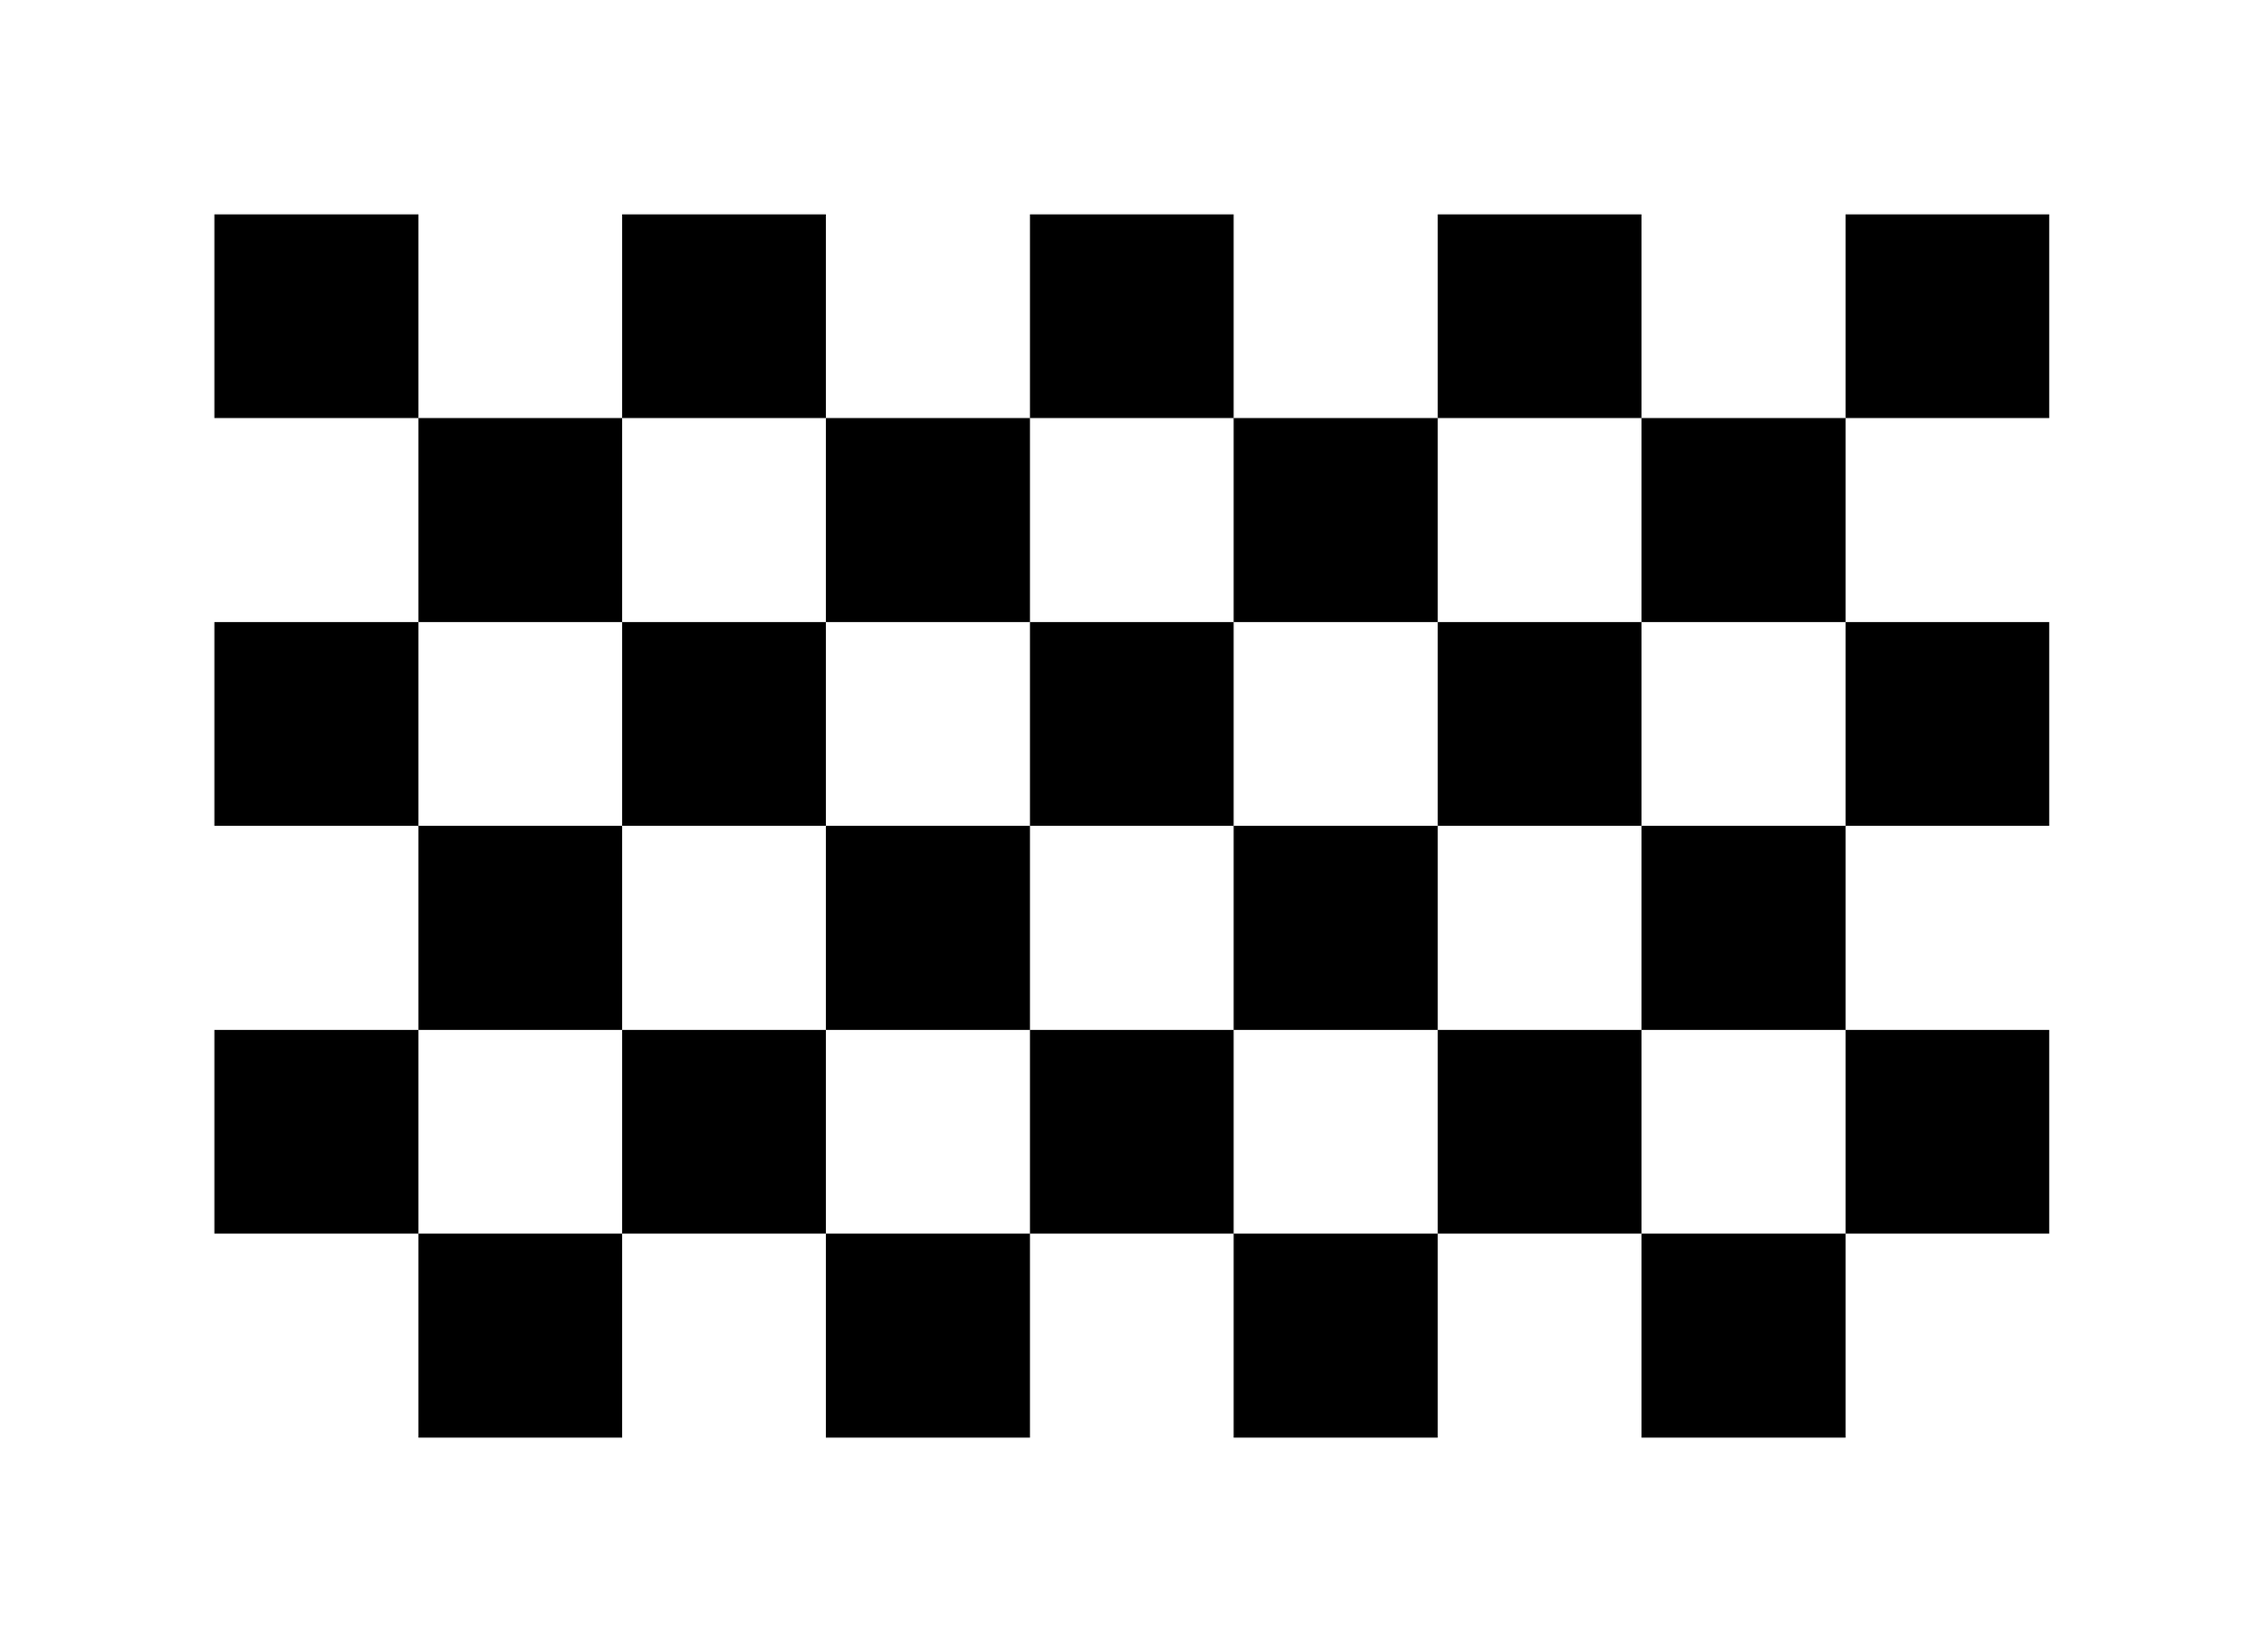
\begin{tikzpicture}[x=\S\U,y=\S\U]
\fill[bgcolor] (0,0) rectangle (\N+3,\M+3);
\ifprintdims
    \node[align=center,scale=1,text=fgcolor] at (0.5, \M+2.8) 
        {pattern $\N\times\M$/$\S\U$\\total  $\pscalculate{(\N+3) * \S}\U\times\pscalculate{(\M+3)*\S}\U$};
\fi
\begin{scope}[shift={(1,1)}]
\foreach \y in {0,1,...,\numexpr\M}{
    \foreach \x in {0,1,...,\numexpr\N}{
        \pgfmathparse{mod(\x+\y,2) ? "fgcolor" : "bgcolor"}
        \edef\rcolor{\pgfmathresult}
        \fill[\rcolor] (\x ,\y) rectangle (1+\x,1+\y);
}}
\end{scope}
\ifprintcontrols
    \fill[fgcolor] (0,0) rectangle (0.1,0.1);
    \fill[fgcolor] (0,\M+3-0.1) rectangle (0.1,\M+3);
    \fill[fgcolor] (\N+3-0.1,\M+3-0.1) rectangle (\N+3,\M+3);
    \fill[fgcolor] (\N+3-0.1,0) rectangle (\N+3,0.1);
\fi
\end{tikzpicture}
\end{document}
